\chapter{Motors}
\label{chap:motors}

A l’actualitat els motors desenvolupen tasques que simplifiquen molt el dia a dia de les persones. Gràcies als motors, la majoria de tasques que fa un parell de segles es necessitava la força conjunta d’un gran nombre de persones ara ja són els motors qui s’encarreguen d’aquesta feina. Els motors també han suposat un gran avenç en el desplaçament de les persones, abans viatjar era una cosa molt eventual i lenta i ara pots donar la volta al món en menys de 24 hores. Segurament molta gent ja està familiaritzat amb el concepte de motor, encara que mai està de més repassar conceptes.

Un motor és una màquina dissenyada per convertir un tipus d’energia (elèctrica, de combustible fòssils, etc.), en energia mecànica. Aquesta energia mecànica és la que s’aprofita per a generar moviment. 
     
\section{Tipus de motors}
Els motors s’organitzen en funció de la font d’energia que empren per a transformar-la en energia mecànica. A continuació, es veurà de forma resumida els diferents tipus de motors.

\subsection{Motors de gasolina}
Els motors de gasolina són aquells que funcionen amb una base \newline termodinàmica que s’encarrega de convertir l’energia química de la ignició, provocada per la barreja de l’aire i el combustible, en energia\newline mecànica. D’aquesta manera, el vehicle obté l’energia necessària per a realitzar els seus moviments.

\begin{figure}[H]
		\centering
    	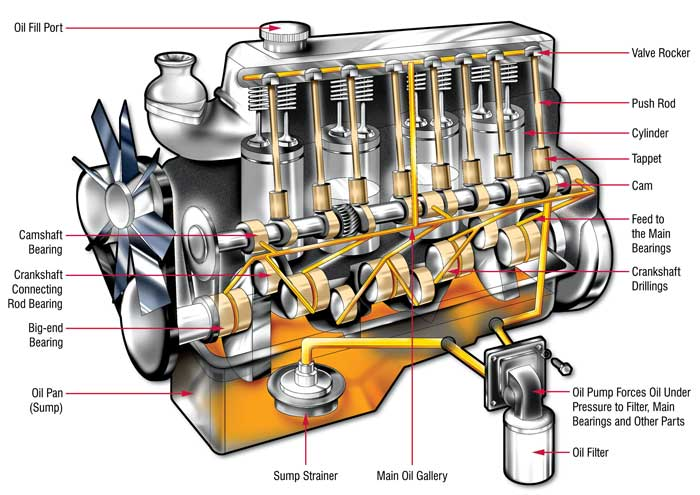
\includegraphics[width=\textwidth, height=8cm]{Motors/motorgasolina.jpg}
     	\caption{Esquema d'un motor de gasolina} 
\end{figure}

Els motors gasolina funcionen en cicles de quatre temps que es podrien classificar, a grans trets, de la següent forma:

\begin{itemize}
  \item Fase d’admissió: La vàlvula d’admissió s’obre, el que permet que la barreja d’aire i combustible flueixi cap a l’interior dels cilindres.
  \item Fase de compressió: Durant aquesta fase, la vàlvula es tanca i el pistó puja per a comprimir la barreja.
  \item Fase d’explosió: Les bugies originen l’espurna necessària per produir l’explosió i el descens dels pistons.
  \item Fase d’escapament: la vàlvula d’escapament s’obre i els pistons \newline s’eleven per expulsar els gasos cremats cap a l’exterior.
\end{itemize}

\subsection{Motors dièsel}
Per norma general, els motors dièsel són principalment emprats en medis de transport que requereixen una dosi extra de potència i que estan pensats per una major càrrega diària de treball, com vehicles industrials, de càrrega, maquinària, medis aeronàutics, etc.
No obstant, des de que aquest tipus de motors naixés de la mà de Rudolf Dièsel en 1893, la tecnologia s’ha estès també cap a medis de transport particulars, arribant actualment a superar en número als vehicles que funcionen amb gasolina.

\begin{figure}[H]
		\centering
    	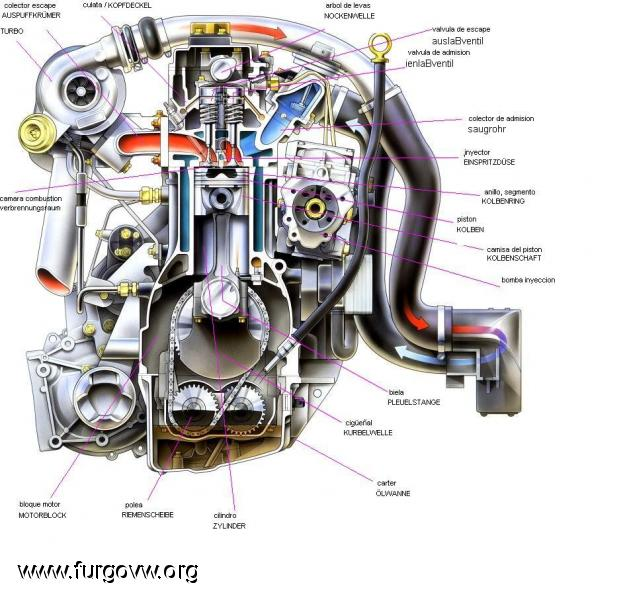
\includegraphics[width=8cm, height=8cm]{Motors/motordiesel.jpg}
     	\caption{Esquema d'un motor diésel} 
\end{figure}

Els motors dièsel funcionen de manera similar als de gasolina i el \newline seu  procés pot dividir-se és d’igual forma en quatre temps, que són els següents:

\begin{itemize}
 		\item Fase d’admissió: Es produeix l'ompliment d’aire i la vàlvula \newline d’admissió roman oberta mentre el pistó descendeix fins el punt\newline mort inferior.
  		\item Fase de compressió: La vàlvula d’admissió es tanca quan el pistó arriba al punt mort inferior i comença el recorregut fins al superior, comprimint l’aire que es troba dintre del cilindre.
  		\item Fase de combustió: L’injector polvoritza el combustible dins de \newline la  càmera i aquest s’inflama d’immediat a l’entrar en contacte amb \newline l’aire  calent.
  		\item Fase d’escapament: S’expulsen els gasos cremats i es deixa que la inèrcia torni a iniciar el cicle.
\end{itemize}

\subsection{Motors de GLP i GNC}
Els vehicles que funcionen amb combustibles alternatius com el GLP (gas liquat del petroli) o el GNC ( gas natural comprimit) van guanyant terreny en la indústria automobilística, i cada cop són més els fabricants que aposten per comercialitzar versions d’alguns dels seus models, propulsats per aquest tipus de combustibles.

\begin{figure}[H]
		\centering
    	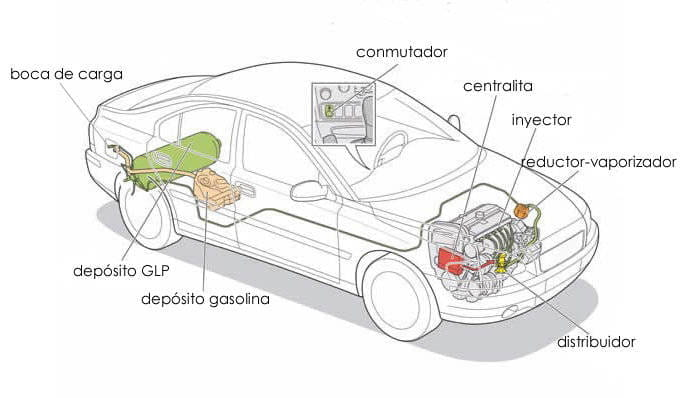
\includegraphics[width=\textwidth, height=8cm]{Motors/motorgnc.jpg}
     	\caption{Esquema de motor gas/gasolina} 
\end{figure}

Qualsevol de les dues opcions, GLP o GNC, afavoreixen l’augment de la vida útil del motor, ja que no generen tant desgast en els cilindres i es depositen menys residus en el sistema. No obstant, s’ha de tindre en compte que en ocasions dificulta la lubricació i pot deteriorar les vàlvules a major velocitat, cosa que podem solucionar gràcies a la mecànica preventiva i realitzant un bon manteniment. 

\subsection{Motors elèctrics}
Encara que no ho sembli, els motors elèctrics són anteriors als dièsel o gasolina de quatre temps. Al 1832 Robert Anderson va desenvolupar el primer automòbil amb motor elèctric pur, capaç de transformar l’energia elèctrica en energia mecànica per medi dels camps magnètics que genera, sense necessitat d’explosions ni combustions pròpies dels motors gasolina i dièsel.

\begin{figure}[H]
		\centering
    	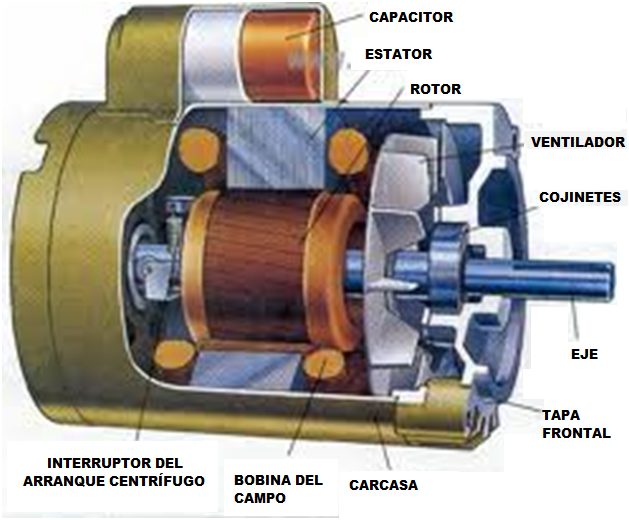
\includegraphics[width=\textwidth, height=8cm]{Motors/motorelectrico.png}
     	\caption{Esquema de motor elèctric} 
\end{figure}

En l’actualitat quan pensem en vehicles elèctrics purs, normalment ens referim a BEV, o vehicles elèctrics de bateria. No obstant, en el mercat podem trobar altres opcions com els FCEV, de pila de combustible, que van combinats amb hidrogen i els HEV i PHEV, coneguts com híbrids i endollables respectivament, que alternen un motor elèctric d’imant permanent amb un de combustió interna (de gasolina principalment). Ja que el nostre controlador serà per a vehicles elèctriques, vol dir que el motor ha de funcionar amb electricitat i per tant, aquest serà el tipus de motor en el qual hi treballarem.

\section{Motors elèctrics}
Els motors elèctrics són màquines elèctriques rotatòries. Transformen una energia elèctrica en energia mecànica de rotació en un eix. Tenen múltiples avantatges, entre els quals cap citar la seva economia, neteja, comoditat i seguretat de funcionament, el motor elèctric ha reemplaçat en gran part a altres fonts d’energia, tant en la indústria com en el transport, les mines, el comerç o la llar.

El seu funcionament es basa en les forces d’atracció i repulsió establertes entre un imant i un fil (bobina) per on circularà un corrent elèctric. Aleshores només serà necessari una bobina (espires amb un principi i fi) un imant i una pila (per a fer passar el corrent elèctric per les espires) per construir un motor elèctric. Per a entendre-ho millor cal saber com funciona l'electromagnetisme.

L'electromagnetisme és la part de la física que estudia les relacions entre el magnetisme i l'electricitat. L'espai on existeixen les forces magnètiques s'anomena camp magnètic. Un camp magnètic el pot generar un imant amb dos pols, pol Nord (N) i pol sud (S). Aquests pols es troben en els extrems del camp que genera l’imant.

\begin{figure}[H]
		\centering
    	
\includegraphics[width=\textwidth, height=8cm]{Motors/campomagnetico.png}
     	\caption{Funcionament del camp magnètic} 
\end{figure}

Tot imant té un camp magnètic i quan el travessa un altre camp magnètic, el d’un altre imant per exemple, els imants es mouen per atracció o repulsió. Si s’apropen dos imants, quan s'ajuntin els camps magnètics generats per cada un d’ells, es mouran. En resum, pols iguals enfrontats es repelen i pols diferents s’atrauen.

No només es pot crear un camp magnètic amb un imant, es pot generar un camp magnètic amb l’electricitat. Les dues forces magnètiques, una del corrent del conductor i l’altre del propi imant, interactuen fent que l’imant giri. En definitiva mitjançant l’electricitat es pot crear el gir d’un eix que en el fons és la funció mecànica que desenvolupen. 

També succeeix al contrari, que es com es construeixen els motors elèctrics de corrent continua.

Si un conductor pel qual circula un corrent elèctric es troba dins d’un camp magnètic, el d’un imant per exemple, el conductor es desplaça perpendicularment al camp magnètic, és a dir, es crea una força en el conductor que fa que aquest es mogui. Realment el corrent que circula pel conductor el que fa és crear al seu voltant un camp magnètic i a l’interactuar el camp de l’imant amb el camp creat en el conductor, es produeix el seu moviment al ser com dos imants. Segons el sentit del corrent del conductor el camp creat tindrà una polaritat o la seva contrària, els camps s’atrauran o repel·liran fent que el conductor es mogui en un sentit o en l’altre.
Si el camp magnètic és horitzontal i el conductor està vertical, el conductor es desplaçarà sortint o entrant de l’imant que provocarà el camp magnètic (depèn del sentit de la corrent pel conductor).

Un cop vists els principis bàsics de funcionament de qualsevol motor \newline elèctric, es mostraran els diferents tipus per tal de veure amb una visió molt major quin seria l'ideal per a enfocar el controlador de vehicles \newline elèctrics per aquest tipus de motor.

\section{Motor de corrent continu}

Van ser els primers en fer-se servir en vehicles elèctrics per les seves bones característiques en tracció i per la simplicitat dels sistemes de control de l'electricitat des de les bateries. Presenten desavantatges en quant al manteniment d'algunes de les peces (escombretes i col·lectors) ja que són motors grans si es busquen potències elevades, doncs la seva estructura (i en concret el fregament entre peces) condiciona el límit de velocitat de rotació màxima. 

Els motors de corrent continu s'utilitzen en casos on és important poder regular contínuament la velocitat del motor, a més a més, s'utilitzen en aquells casos on és imprescindible fer servir corrent directe, com en el cas de motors accionats per piles o bateries. Aquests tipus de motors han de tenir en el rotor i l'estator el mateix nombre de pols i el mateix nombre d'escombretes. Aquests motors poden ser de tres tipus: Sèrie, paral·lel o mixt. 

\begin{itemize}
    \item Motor sèrie: és un tipus de motor elèctric de corrent continu en el qual el bobinat de camp (camp magnètic principal) es connecta en sèrie amb l'armadura.
    \item Motor Paral·lel: és un motor de corrent continu on el bobinat inductor principal està connectat en derivació amb el circuit format pels bobinats induïts e inductor auxiliar.
    \item Motor compost: és un motor de corrent continu on la seva \newline excitació es originada per dues bobines inductores independents; una disposada en sèrie amb el bobinat induït i un altre connectat en derivació amb el circuit format pels bobinats induïts, inductor sèrie i inductor auxiliar. Els motors composats tenen un camp sèrie sobre el límit del bobinat del camp paral·lel. 
\end{itemize}

\subsubsection{Composició}
En primera instància és fonamental senyalar que un motor de corrent continu està composat a grans trets per dues parts. Un estator amb el que se li dóna suport mecànic a l'aparell i és on s'ubiquen els pols de la màquina, que és on quedaran bobinats de fil de coure sobre un nucli de ferro o imants permanents.

Per altra banda està el rotor que quasi sempre és de forma cilíndrica, el qual també està bobinat i amb nucli i s'alimenta amb corrent directe per medi de delgues, les quals estan en contacte de manera alterna amb escombretes fixes.

A mode de resum, en el moment en que un conductor, pel qual està passant corrent elèctrica és submergit en un camp magnètic, aquest conductor sofrirà una força perpendicular al pla que es forma pel camp magnètic i la corrent.

\begin{figure}[H]
		\centering
    	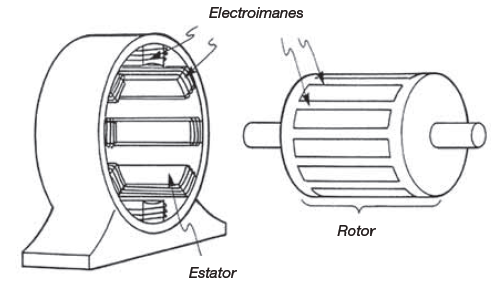
\includegraphics[width=\textwidth, height=8cm]{Motors/rotorestator.png}
     	\caption{Composició d'un motor elèctric de corrent continu}
\end{figure}

\subsubsection{Avantatges}
Encara que el preu d'un motor de corrent continu és considerablement major que el d'un motor d'inducció d'igual potència, existeix una tendència creixent a fer servir motors de corrent continu en aplicacions especials.

La gran varietat de la velocitat, juntament amb la seva facilitat de control i la gran flexibilitat de les característiques par-velocitat del motor de corrent continu, han fet que en els últims anys es faci servir cada cop més amb màquines de velocitat variables en les que es necessiti ampli marge de velocitat i control de les mateixes.

Existeix un creixent número de processos industrials que requereixen una exactitud en el seu control o una gama de velocitats que no es pugui aconseguir amb motors de corrent altern. El motor de corrent continu manté un rendiment alt en un ampli marge de velocitats, el que juntament amb la seva alta capacitat de sobrecàrrega, el fa més apropiat que el de corrent altern per a moltes aplicacions.

\subsubsection{Funcionament}
Quan el corrent passa a través del rotor d'un motor de corrent continu, es genera un par de forces, per la reacció magnètica, i el rotor gira. L'acció del commutador i de les connexions de les bobines del camp dels motors són exactament les mateixes que fan servir els generadors. La revolució del rotor indueix un voltatge en les bobines d'aquesta. Aquest voltatge és oposat en la direcció al voltatge exterior que s'aplica al rotor, i d'allà que es coneixen com voltatge induït o força contraelectromotriu. 

Quan el motor gira més ràpid, el voltatge augmenta fins que és quasi igual a l'aplicat. El corrent aleshores és petit, i la velocitat del motor romandrà constant sempre que el motor no estigui sota càrrega i tingui que realitzar un altre treball mecànic que no sigui el requerit per moure el rotor. Sota càrrega, el rotor gira més lentament, reduint el voltatge induït i permetent que flueixi un corrent major en el rotor. El motor pot així rebre més potència elèctrica de la font, subministrant-la i fent més treball mecànic.

La velocitat a la que funciona un motor depèn de la intensitat del camp magnètic que actua sobre el rotor, així com del corrent d'aquest. Quant més fort és el camp, més baix és el grau de rotació necessari per generar un voltatge induït prou gran com per contrarestar el voltatge aplicat. Per aquesta raó, la velocitat dels motors de corrent continu pot controlar-se mitjançant la variació del corrent del camp.

\begin{figure}[H]
		\centering
    	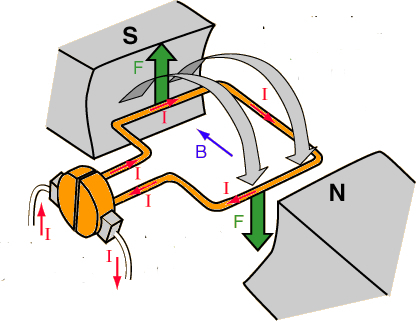
\includegraphics[width=\textwidth, height=8cm]{Motors/funcmotorcontinua.jpg}
     	\caption{Funcionament d'un motor de corrent continu.} 
\end{figure}

En la figura anterior s'explica gràficament el seu funcionament. Es pot apreciar com en el rotor el corrent entra per la part esquerra i per la polarització de l'imant extern fa que el rotor giri en sentit horari. En la següent imatge es pot apreciar les diferents posicions que pot agafar el motor.

\begin{figure}[H]
		\centering
    	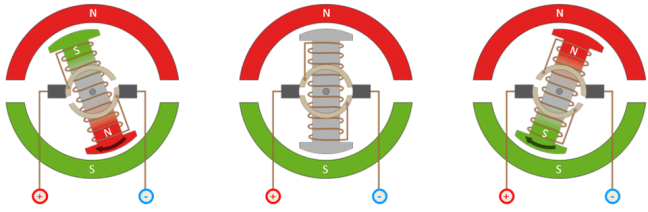
\includegraphics[width=\textwidth, height=6.5cm]{Motors/motorcontinua.png}
     	\caption{Posicions d'un motor de corrent continu.} 
\end{figure}

Els motors de corrent continu són alguns dels motors elèctrics més potents i flexibles. S'utilitzen en ventiladors, arrancadors elèctrics i molts altres aparells. Un motor sèrie DC s'anomena així perquè la bobina de camp i la bobina de rotor estan ambdues connectades en sèrie una amb l'altra. En aquesta configuració el mateixa corrent flueix a través d'ambdues bobines

\subsection{Motors sèrie}
La idea d'aquests tipus de motors és que es connecten a la càrrega en sèrie. El voltatge que s'aplica és constant, mentre que el camp d'excitació augmenta amb la càrrega, donat que el corrent és el mateix corrent d'excitació.

La rotació es pot invertir canviant la direcció del corrent, ja sigui del camp en sèrie o de l'induït.

\begin{figure}[H]
		\centering
    	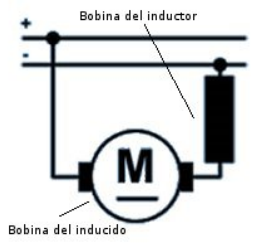
\includegraphics[width=7cm, height=7cm]{Motors/motordcserie.png}
     	\caption{Esquema d'un motor CC en sèrie.} 
\end{figure}

El par produït és directament proporcional al flux i al corrent en l'Induït. El par motor és directament proporcional al quadret de Ia, per tant, la seva corba és parabòlica.

\begin{figure}[H]
		\centering
   	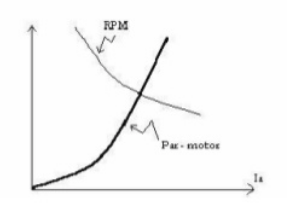
\includegraphics[width=8cm, height=6cm]{Motors/parrpm.png}
     	\caption{Par motor en funció de la intensitat. } 
\end{figure}

\subsubsection{Arrancada i parada del motor}
L'arrancada del motor es produeix intercalant un reòstat d'arrencada en sèrie amb el corrent induït. Aquesta resistència es redueix gradualment quan el motor adquireix velocitat. 

A l'augmentar el corrent per a donar més força a l'arrencada, disminueix la velocitat. Per aquesta raó un motor sèrie ha d'estar sempre engranat o acoplat directament a la càrrega. Si un motor sèrie estigués unit a la càrrega mitjançant una corretja i aquesta es trenqués o es soltés, el motor s'embalaria i molt probablement es danyaria.

Per parar un motor sèrie, és precís introduir progressivament resistències del reòstat d'arrencada i tallar després l'alimentació per evitar un corrent de ruptura agressiu que seria perillós per als enrotllaments

\subsubsection{Velocitat i propietats}
La velocitat es pot variar, canviant el voltatge aplicat, col·locant un reòstat en sèrie amb la bobina de camp. D'aquesta manera es disminueix la velocitat. Es pot augmentar la velocitat, disminuint el flux de corrent per pols. Això es pot realitzar, col·locant un reòstat en paral·lel amb la bobina de camp, de forma que el corrent total només permeti circular una part per la bobina d'excitació.

Les propietats principals d'aquests motors són les següents:
\begin{itemize}
    \item Gran par d'arrencada.
    \item Velocitat variable amb la càrrega.
    \item Tendència a l'accelerament excessiu.
    \item Suporta bé les sobrecàrregues.k
    \item Es dispara fàcilment en el buit o quan la càrrega decreix.
\end{itemize}

Els motors en sèrie tenen aplicacions en aquells casos on es requereix un elevat par d'arrancada a petites velocitats i un par reduït a grans velocitats. El motor ha de tenir càrrega si està en marxa. Alguns exemples serien els tramvies, locomotores, o la majoria de joguines. 

\subsection{Motors paral·lel}

Els trepants són màquines que serveixen per a foradar. Aquestes màquines funcionen amb motors en paral·lel. Però per què? Perquè no poden ser motors en sèrie? Doncs la resposta és evident. En el moment en el que el trepant efectués l'orifici a la peça, la màquina quedaria al buit, és a dir, que no hi hauria cap resistència a la força realitzada al motor. La velocitat a la broca augmentaria tant que arribaria a ser perillós per a l'usuari.

\begin{figure}[H]
		\centering
    	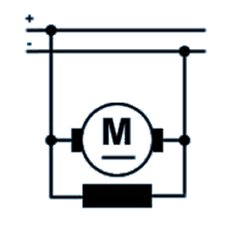
\includegraphics[width=8cm, height=7cm]{Motors/Motor_paralelo.jpg}
     	\caption{Esquema d'un motor CC amb càrrega en paral·lel} 
\end{figure}

Els motors en paral·lel són uns motors on les bobines estan connectades en paral·lel amb les bobines induïdes. D'aquesta forma, de tot el corrent absorbit pel motor, una part circula per les bobines induïdes i l'altra per les inductores. El circuit d'excitació està a la mateixa tensió que l'inductor (ja que un circuit en paral·lel es manté el voltatge però es redueix la intensitat).

El sentit de rotació d'un motor paral·lel es pot invertir, canviant la direcció del corrent, ja sigui en el circuit de camp o en el circuit de l'induït.

Aquest motor es diferencia amb el motor en sèrie per 3 raons principals:
\begin{itemize}
    \item En l'arrancada, el par motor és menor que en el motor sèrie.
    \item Si la intensitat de corrent absorbida disminueix i el motor està en buit, la velocitat de gir nominal quasi no varia. És més estable que el sèrie.
    \item Quan el par motor augmenta, la velocitat de gir quasi no disminueix.
\end{itemize}

Encara que el motor paral·lel és de velocitat constant, la seva característica més important, és la de ser un motor de velocitat regulable. La velocitat pot augmentar disminuint el flux per pols. Per això, és necessari col·locar un reòstat en el circuit de camp. Per parar el motor s'introdueixen totes les resistències del reòstat d'arrancada abans de tallar el corrent.

Les propietats principals d'un motor paral·lel són les següents:
\begin{itemize}
    \item Par d'arrancada feble.
    \item No suporten grans sobrecàrregues.
    \item Velocitat constant en qualsevol càrrega.
    \item No es disparen en el buit.
\end{itemize}

La velocitat constant d'aquests motors els fa adequats per l'accionament de màquines, eines i aparells d'elevació. S'inclouen tots els casos on no es requereixi un par elevat a petites velocitat i no produeixin càrregues grans, si la càrrega desapareix (en el buit) el motor quasi no varia de velocitat.

\subsection{Motor mixt}
El motor mixt és una combinació del motor sèrie i el motor paral·lel,  donat que una de les bobines inductores està en sèrie amb l'induït, mentre que l'altra està en paral·lel amb ell. Una part de la intensitat de corrent absorbit circula per les bobines induïdes i, per tant, per una de les inductores; mentre que la resta del corrent recorre l'altra bobina inductora. 

\begin{figure}[H]
		\centering
    	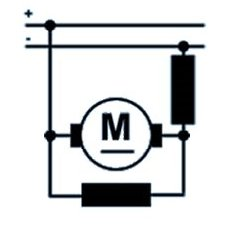
\includegraphics[width=8cm, height=8cm]{Motors/Motor_compuesto.jpg}
     	\caption{Esquema d'un motor CC amb càrrega en paral·lel.} 
\end{figure}

Comparant els avantatges dels motors sèrie i paral·lel es troba que el motor paral·lel té una major velocitat constant, però un motor sèrie de la mateixa capacitat pot exercir un par molt major, quan és necessari, sense augmentar terriblement el corrent. Aquestes dues característiques poden obtindre's en un mateix motor col·locant dos bobinats de camp: Un en sèrie i l'altre en paral·lel en els pols del motor. És per això que es denominen motors mixts. 

La velocitat d'un motor compost es pot disminuir per sota la normal \newline mitjançant un reòstat col·locat en el circuit de l'induït i augmentar per sobre de la normal mitjançant un reòstat en el circuit de camp. A diferència dels motors en sèrie, el motor compost té una velocitat definida sense càrrega i no arribarà a velocitats destructives si aquesta es suprimeix. La regulació de la velocitat és inferior a la d'un motor paral·lel i major a la d'un sèrie. La rotació s'inverteix canviant la direcció del corrent del circuit de camp o del circuit induït. Donat que si s'inverteix el camp paral·lel s'ha d'invertir el sèrie, el procediment més simple és invertir el corrent en l'induït.

\section{Motor de corrent altern}

Es denomina motor de corrent altern aquells motors elèctrics que funcionen amb corrent altern. Un motor és una màquina motriu, això és, un aparell que converteix una forma determinada d'energia en energia mecànica de rotació o par. Un motor elèctric converteix l'energia elèctrica en força de gir per mitjà de l'acció mútua dels camps magnètics.

Els motors de corrent altern es classifiquen per la seva velocitat de gir, pel tipus de rotor i pel nombre de fases d'alimentació:
Existeixen 4 tipus:

\begin{itemize}
    \item Motor universal: Pot treballar tant en CA com en CC: L'ús d'aquests motors en corrent altern està molt estès pel major par d'arrancada respecte al dels motors d'inducció i per la seva elevada velocitat de rotació, el que permet reduir la seva mida i el seu preu. Així, s'empren en màquines com eines portàtils de tot tipus, \newline electrodomèstics petits, etc.
    \item Motor asíncron: Són un tipus de motor de corrent altern en el que el corrent elèctric, en el rotor, necessari per produir torsió és induït per inducció electromagnètica del camp magnètic de la bobina de l'estator. Per tant un motor d'inducció no requereix una commutació mecànica apart de la seva mateixa excitació o per tota o part de l'energia transferia de l'estator al rotor, com en els universals, DC i motors grans síncrons.
    \item Motor síncron: Els motors síncrons són un tipus de motor de corrent alterna en el que la rotació de l'eix està sincronitzada amb la freqüència del corrent d'alimentació; el període de rotació és exactament igual a un nombre enter de cicles de CA.
    \item Motor de gàbia d'esquirol: La major part dels motors que funcionen amb CA d'una sola fase tenen el rotor de tipus gàbia d'esquirol. Els rotors de gàbia d'esquirol reals són molt més compactes i tenen un nucli de ferro laminat.
\end{itemize}

\subsubsection{Composició}

De la mateixa forma que amb els motors de corrent continu, aquests motors estan composats a grans trets per dos components principals: el rotor i l'estator. 

El circuit magnètic dels motors elèctrics de corrent altern està format per xapes magnètiques i aïllades entre elles per eliminar el magnetisme permanent.

El circuit magnètic està forma per xapes apilades en forma de cilindre en el rotor i en forma d'anell a l'estator. El cilindre s'introdueix a l'interior de l'anell. L'anell es dota de ranures en la seva part interior per col·locar el bobinat inductor i s'embolica exteriorment per una peça metàl·lica amb suport, la carcassa.

\subsection{Motor universal}
S'anomena així per ser l'únic motor que pot connectar-se tant a corrent altern com a corrent continu. Quan el motor es connecta al corrent continu amb una càrrega constant, la velocitat i la potència augmenten proporcionalment amb el voltatge aplicat.

Quan aquest motor es connecta al corrent altern amb càrrega constant, la velocitat i la potència augmenten proporcionalment amb el voltatge aplicat.

En el motor universal la velocitat donada per un voltatge en corrent altern és inferior que la que s'obtindrà si s'aplica el mateix voltatge però en corrent continu. Els motors universals es construeixen per potències menors a mig cavall de potència i velocitats de fins a 3000 rpm i presenten un bon rendiment.

El principi de funcionament d'aquest motor elèctric està determinat per l'efecte motor que produeix un conductor recorregut per un corrent \newline elèctric i que està sotmès a un camp magnètic. Per acció magnetomotriu existirà un desplaçament i per tant es produirà una rotació.

El motor universal està composat pels següents components:
\begin{itemize}
    \item Bobines conductores.
    \item Bobines induïdes.
    \item Escombretes.
    \item Ressorts.
    \item Tapes o escuts.
\end{itemize}

\begin{figure}[H]
		\centering
    	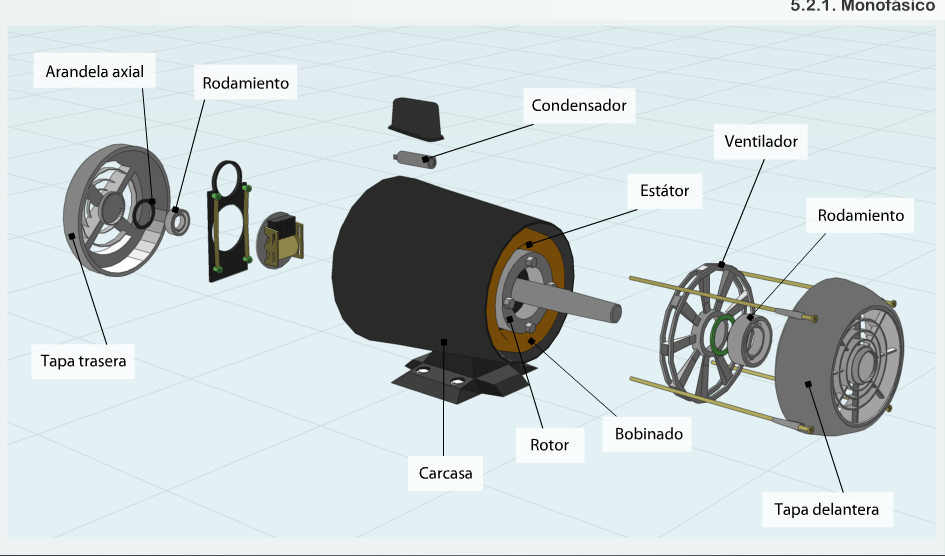
\includegraphics[width=\textwidth,height=8cm]{Motors/composicionmotoruniversal.png}
     	\caption{Constitució d'un motor universal.} 
\end{figure}

Les característiques principals d'aquests tipus de motos són les següents:
\begin{itemize}
    \item Funciona amb corrent altern i corrent directe.
    \item Posseeix un par d'arrancada molt elevat.
    \item Per invertir el sentit de rotació, s'inverteix el sentit del corrent en qualsevol dels bobinats.
\end{itemize}

El motor elèctric basa el seu funcionament en la llei de Laplace. El bobinat inductor i el bobinat induït estan connectats en sèrie. Al ser recorreguts per un corrent, el bobinat inductor forma el camp magnètic i l'induït per la llei de Laplace, al ser recorregut pel corrent i sotmès a la influència del camp magnètic inductor, es desplaça, donant origen al gir del rotor.

Si augmenta el camp augmenta la força i la velocitat. El camp magnètic que produeix la bobina induïda provoca una deformació del flux inductor anomenat reacció de l'inductor. En corrent altern o en corrent continu el sentit es manté per l'acció de cada alternança en particular. En corrent altern es produeix una força contraelectromotriu per efecte transformador i per efecte generador. En corrent continu només per efecte generador.

Com en la majoria de motors la regulació es pot establir mitjançant reòstats o per commutació de resistències

\subsection{Motor síncron}
Una màquina sincrònica és una màquina de corrent altern on la seva velocitat és proporcional a la freqüència del corrent. El camp magnètic que creen els corrents de l'armadura gira a la mateixa velocitat que el que crea el corrent de camp en el rotor, i es produeix un par estacionari.

Aquests motors són màquines rotatòries elèctriques que poden treballar tant com motor com generador. Com a motor es converteix l'energia \newline elèctrica en energia mecànica i viceversa com a generador. Aquestes \newline màquines no tenen par d'arrancada i s'ha d'emprar diferents mètodes d'arrancada i acceleració fins la velocitat nominal de sincronisme.

Les màquines sincròniques s'utilitzen en major mesura com generadors de corrent continu que com motors de corrent altern. La màquina tipus síncrona més estesa és l'alternador, que és l'aparell que s'encarrega \newline d'aprofitar l'energia mecànica que genera un cotxe i convertir-la en energia elèctrica per a carregar la bateria del propi cotxe.

\begin{figure}[H]
		\centering
    	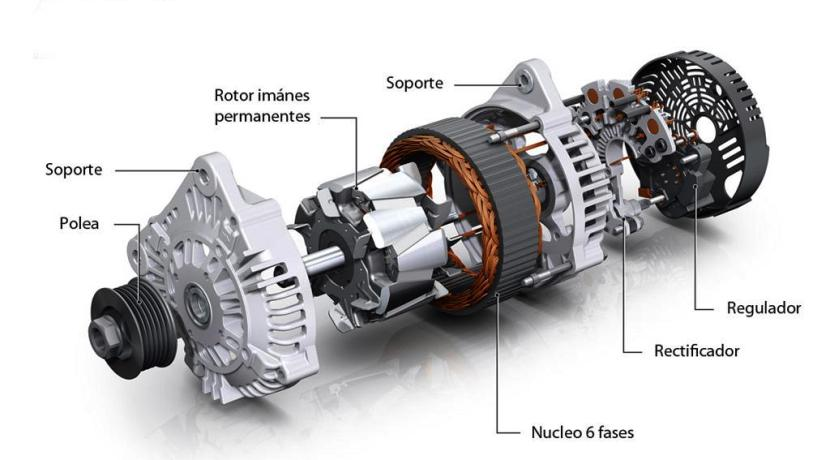
\includegraphics[width=\textwidth,height=8cm]{Motors/alternador.jpg}
     	\caption{Esquema d'un alternador.} 
\end{figure}


A nivells de construcció, són molt similars a la majoria de motors, formant-se per un rotor i un estator. L'estator és completament igual que el d'un motor asíncron però és al rotor on hi apareixen certes diferències. Aquest rotor conté un debanament de corrent continu, denominat debanament de camp i un debanat en curtcircuit, que impedeix el funcionament de la màquina a una velocitat diferent a la de sincronisme, denominat debanament amortidor. A més a més, conté un circuit magnètic format per apilament de xapes magnètiques de menor gruix que les de l'estator.

Les principals avantatges que presenten són les següents:
\begin{itemize}
    \item És l'única màquina que ofereix garantia en la estabilitat de la velocitat.
    \item Tenen un molt bon rendiment.
    \item Poden fer-se servir com a dispositius de correcció del factor de \newline potència. El factor de potència es controla variant l'excitació del rotor.
    \item Poden ser connectats directament a una xarxa d'alta tensió sense necessitat de transformador intermedi.
    \item Possibilitat de funcionar com generador de potència reactiva.
    \item Subministrament de potència a càrregues que treballen a velocitat constant.
    \item El voltatge en els terminals i la freqüència del sistema seran constants, independentment de la quantitat de potència presa pel motor.
\end{itemize}

Per entendre millor el funcionament dels motors síncrons cal tenir clar que la velocitat és proporcional a la freqüència del corrent de l'armadura i que el camp magnètic creat pels corrents de l'armadura giren a la mateixa velocitat que el que crea el corrent de camp en el rotor. 

Els pols del rotor estan sotmesos a atraccions i repulsions, en breus \newline períodes de temps, per part dels pols de l'estator, però el rotor no aconsegueix girar fins arribar a la velocitat de sincronisme. 

\begin{figure}[H]
		\centering
    	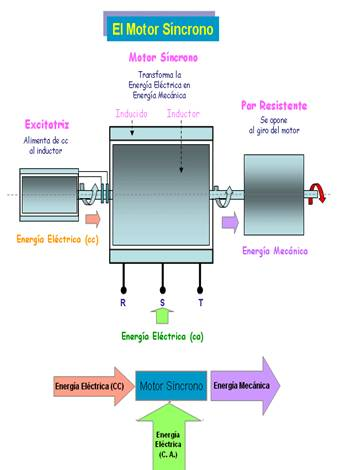
\includegraphics[width=8cm,height=8cm]{Motors/funcionamientomotorsincrono.jpg}
     	\caption{Funcionament d'un motor síncron.}
\end{figure}

\subsection{Motor asíncron}
Els motors asíncrons o d'inducció són motors de corrent altern en els que el corrent elèctric que es necessita per produir la torsió del rotor és induïda per inducció electromagnètica del camp magnètic de la bobina de l'estator. D'aquesta forma, els motors asíncrons no necessiten una commutació \newline mecànica com succeeix en els motors síncrons i els motors de corrent continu.

Els motors asíncrons estan constituïts principalment per dues parts: 
\begin{itemize}
    \item Circuit magnètic: La part fixa del circuit magnètic (estator) és un anell cilíndric de xapa magnètica ajustada a la carcassa que l'envolta. La carcassa té una funció purament protectora. 
    \item Circuits elèctrics: Els dos circuits elèctrics van situats un en les ranures de l'estator i l'altre en les del rotor, que està curtcircuitat. 
\end{itemize}

\subsection{Motor pas a pas}
Els motors pas a pas són un tipus especial de motors que permeten l'avenç del seu eix en angles molt precisos i per passos en les dues possibles direccions de moviment. Aplicant a ells una determinada seqüència de senyals digitals, avancen per passos cap a un costat o l'altre i es detenen exactament a una determinada posició.

Cada pas té un angle molt precís determinat per la construcció del motor, el que permet realitzar moviments exactes sense necessitat d'un sistema de control de llaç tancat.

A un motor pas a pas se li pot ordenar per medi del control, que avanci cinc o deu passos cap a la dreta, després un determinat nombre de passos cap enrere o simplement que no giri, el qual permet el control de la posició, velocitat i sentit. Aquest sistema ha simplificat enormement la implementació \newline d'automatismes i les aplicacions de la robòtica.

Els motors pas a pas presenten grans avantatges respecte a la utilització de servomotors degut a que es poden manejar digitalment sense realimentació, la seva velocitat es pot controlar fàcilment, tenen una llarga vida, són de baix cost, la interfície és senzilla i el seu manteniment és mínim degut a que no tenen escombretes.

El funcionament dels motors pas a pas es basa en el simple principi \newline d'atracció i repulsió que succeeix entre els pols magnètics. 

Per aconseguir un moviment molt més suau, els motors pas a pas es fabriquen augmentant el nombre de pols de l'estator amb una sèrie de ranures tant en el rotor com en l'estator. Així s'aconsegueixen moviments que van fins a 1.8º/pas. Els graus d'avenç per pas són una de les característiques més important en aquest tipus de motors i generalment està indicada en el seu cos.

Els motors PAP tant unipolars com bipolars poden treballar en dos modes d'operació: de pas complert i de mig pas.

En el primer cas, amb cada seqüència el rotor gira un determinat angle donat per la fabricació del motor. En el mode de mig pas, cada seqüència produeix un gir en graus corresponent a la meitat del seu pas normal. 



\subsection{Motor d'imants permanents}
En general el camp magnètic d'un motor DC es pot produir per bobines o imants permanents. Els motors DC d'imant permanents es poden classificar dacord amb l'esquema de commutació i al disseny de l'armadura. Els motors DC convencionals tenen escombretes mecàniques i commutadors. No obstant, en una clase importants de DC la commutació es fa de forma electrònica; aquest tipus de motor s'anomena motor DC sense escombretes.

El flux magnètic produït per l'imant passa a través de l'estructura del rotor laminat amb ranures. Els conductors de l'armadura estan localitzats en les ranures del rotor. Aquest tipus de motor està caracteritzat per una inèrcia del motor relativament alta (ja que la part giratòria està formada per les bobines de l'armadura), una inducció alta, baix cost i alta confiabilitat.

Els conductors de l'armadura estan enganxats a la superfície de \newline l'estructura cilíndrica del rotor, la qual està feta de discs laminats agafats a l'eix del motor. Ja que en aquest disseny no s'empren ranures sobre el rotor, no presenta l'efecte de "roda dentada". Donat que els conductors estan projectats en el entreferro d'aire que està entre el rotor i el camp d'imants permanents, aquest camp té menor inductància que el d'estructura de nucli de ferro.

\section{Motors Brushless}
Els motors brushless són uns motors trifàsics que funcionen mitjançant la commutació de les bobines per el controlador, això ens dóna pràcticament il·limitades revolucions ja que no es limiten unes escombretes a l'hora de commutar las bobines del rotor i estator. Aquests motors necessiten poc manteniment ja que no hi ha peces sotmeses a desgast pel fregament. Tenen una corba de velocitat par plana i poden realitzar el seu par en pràcticament totes les revolucions que en permet el motor. El fet de no tenir baixades de voltatge per la commutació les bobines i el bobinat en l'estator, permet obtenir motors molt més petits amb la mateixa potència. El control de motor es complica ja que la commutació de les bobines es fa mitjançant el controlador i no mecànicament. El fet de ser un motor complex suposa un cost de la construcció del motor i fa que sigui un motor car ja que conté un rotor d'imants permanents.

\subsection{Paràmetres dels motors brushless}

Paràmetres a tenir en compte del motor brushless per fer una selecció correcta del motor que necessitem:\smallskip

\subsubsection{KV}
És un dels paràmetres més importants per la selecció del motor, tot i que en el marcat trobem motors amb la mateixa potència, voltatge i intensitat, però amb diferents KV. A termes generals són les voltes per voltatge que té el motor, es a dir, pel mateix motor les baixes versions de KV tenen més bobinats amb filferro més prim, mentre que les altes versions de KV tenen menys bobines amb filferro més gruixut. Sempre que tinguin la mateixa massa de coure, són exactament iguals pel que fa a la potència màxima de sortida, parell, eficiència i revolucions màximes.\smallskip
    
Poden haver diferents versions KV del mateix motor ja que són totalment equivalents. El KV només afecta al sistema de control i de bateria i per tant, mentre comparem els motors, permet parlar de parell en comptes de corrent perquè el parell és proporcional al corrent / KV i, el valor de KV es pot canviar lliurement amb la quantitat de voltes i el gruix del coure.\bigskip
     
\subsubsection{Sensored i Sensorless}

Depenen de com dissenyem el controlador podrem controlar els motors Sensorless o Sensored o els dos, per això cal veure com funciona l'excitació de les bobines del motor brushless.\smallskip
    
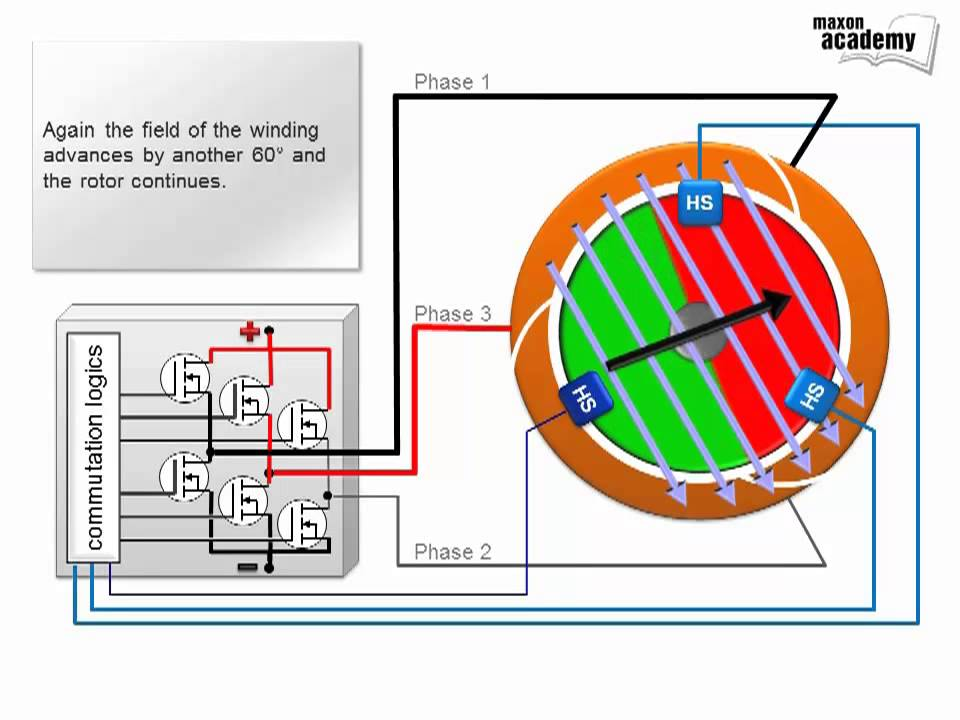
\includegraphics[width=\textwidth]{bobinas}
    
En la imatge es pot veure l¡esquema d'un motor Sensored en el qual porta 3 sensors d'efecte hall per tal de veure el camp magnètic del rotor. A partir d'aquesta informació es pot saber quina orientació té el motor respecte el camp generat per les bobines i alternar a la següent bobina per continuar el gir en la posició òptima. En el cas del Sensorless que no disposa dels sensors d'efecte hall es farà una estimació a partir de la intensitat consumida i els polsos enviats anteriorment. A altes velocitats de rotació l'efecte es poc pronunciat però a baixes velocitats és molt probable que no s'estigui optimitzant el consum del motor ja que s'alterna abans o després del punt ideal de les bobines. Això provocarà un consum extra de potència en les bateries, arribant a sobreescalfar els controlador del motor. 

\subsection{Com funciona el motor Brushless}
Com el seu nom indica són motors sense escombretes, en aquest tipus de motor la corrent passa directament per les bobines creant un camp magnètic que interacciona amb el camp creat pels imants permanents del rotor, per tant el control de les bobines generen el camp i com el movem per produir el gir desitjat el deleguem al variador, per això els sistemes de control són més complicats. Aquest és capaç per uns sensors o pel comportament del corrent determinar la posició magnètica del rotor i modificar el camp magnètic generat per obtenir la força de gir desitjada.
    
Per aconseguir que el motor comenci a girar ha d'induir un camp \newline magnètic a les bobines perpendicular al camp dels imants del rotor, en aquestes condicions el par serà el màxim, és el que en interessa en tot moment, si en algun moment volguéssim menor par disminuiríem la potència del camp però intentaríem fer servir el màxim perpendicularment possible per fer-ho al màxim de eficient.\smallskip
    
En tot moment la posició del rotor és variable, per tant ens hem de dotar de sistemes que ens facilitin saber la posició del rotor per saber com s'han d'excitar les bobines. Aquí disposem de dos estratègies; sensorless (sense sensors) o sensored (amb sensors). Els motors sensored disposen \newline d'elements que ens informen de la posició del camp magnètic o orientació del rotor en tot moment. En el cas dels motors sensorless no es disposa de cap sistema que mostri la posició del camp, normalment es mesuraran els polsos d'intensitat i veient com es comporten es suposarà l'orientació del rotor. Solen ser sistemes més econòmics ja que no tenen un cost de sensors.

\section{Control de motors elèctrics}

Depenen del tipus de motor que tinguem tindrem mesures de control diferents per adaptar-se al motor en qüestió. Dintre de cada tipus de control de motor té diverses formes de ser controlat per tal de simplificar la instal·lació limitant el control d'aquest o controlant tots els aspectes del propi motor. 

Per a parlar dels algorismes de control primerament cal fer una gran diferenciació dels dos grups que hi apareixen; els de llaç obert i els de llaç tancat. La diferència és que els primers no tenen realimentació a un control i els segons sí. Cal veure que depenen del tipus de motor el control amb llaç obert o tancat proporcionarà diferents efectes. 

En el llaç obert nomes apliquem una consigna a la nostra sortida i no tenim en compte que a la realitat aquesta consigna no es realitzi i per tant, s'estigui realitzant un moviment incorrecte. Només es pot confiar en la consigna donada.

En el control de llaç tancat es munta algun tipus de sensor que torna a enviar a un control la informació que realment està reben el motor. Pot ser la velocitat, la intensitat, el parell o la posició. En aquest control si es dóna una ordre X i ens retorna un valor de X-2, el següent enviament enviarem X+2 per compensar aquesta variació. D'aquesta forma és molt més precís aconseguir aquesta consigna.

Els algorismes de control que es tractaran seran els algorismes de llaç tancat, concretament els que es basen en motors amb PID.

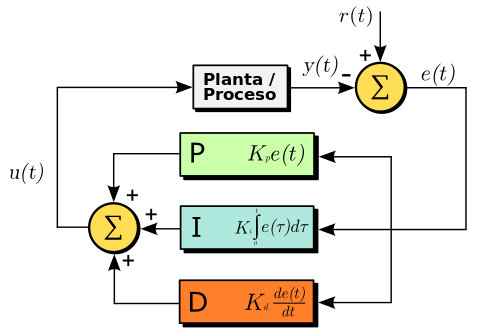
\includegraphics[width=\textwidth]{Motors/PID}

El PID està format per 3 etapes principals les quals són les que es troben si es desglossa l'acrònim PID; Proporcional, Integral i Derivatiu.

Es basa en agafar la resposta del sensor i restar-la a la consigna, aplicant les 3 etapes per donar el senyal més precís al motor, per aconseguir la consigna. El paper que juguen en el control es mostra en els següents punts: 

\begin{itemize}
    \item Proporcional: El control proporcional es basa en multiplicar l'error per una constant per determinar la sortida, és a dir, si estem molt lluny de les consignes donarà una sortida molt gran per aproximar-nos al senyal de referència, però un cop estiguen en aquesta pararà el control donant sortida 0. Això es pot provar una oscil·lació si el valor és molt gran o una no correcció ja que ha de mantenir un error constant per tal d'adaptar-se a la mesura.
    
    \item Integral: Con el seu nom indica es basa en realitzar la integral del senyal d'error. En el cas anterior l'error es manté constant en un valor concret. El control integratiu anirà pujant de valor fins a corregir el problema, és un control que si no es limita provoca moltes oscil·lacions en el control. 
    
    \item Derivatiu: És el que realitza la derivada de l'error per tal de controla el motor. És un control útil en el cas de pertorbacions externes, és a dir, en el cas que arribi una pertorbació externa que es desvia de l'objectiu la derivada corregirà molt i provocarà ràpides i curtes reaccions en el control per tal d'intentar tornar el com mantenint la posició.
\end{itemize}    
    
\subsubsection{Generació d'un senyal PWM}
Una ona PWM es pot generar de forma digital o amb circuiteria electrònica. El més utilitzat és la forma digital amb microcontroladors per tal de facilitar el control. El seu funcionament es basa en un comptador del microcontrolador que es programa de forma que vagi incrementant un valor fins arribar al màxim i que torni a començar pel 0. Això ens donarà el període del senyal PWM. Una vegada tenim el període ens falta el temps d'ON, això ho regularem amb una variable que es compararà amb un valor de temps. Sempre que estigui per sobre engegarem la sortida, això ens provoca que puguem canviar la consigna en tot moment arribant a generar polsos estranys, per això el que farem serà que la consigna només es pugui canviar en el punt més alt o ms baix del comptador.

\subsection{Motor de CC amb escombretes }

Aquests tipus de motors són motors que la seva velocitat depèn directament del voltatge es es posi en els seus terminals i el seu parell depèn del propi motor i de la intensitat que hi circula.

Per un control senzill d'aquest tipus de motors és realitza mitjançant un interruptor, o un relé o un transistor que permetrà controlar el motor en un sentit determinat a la velocitat determinada. No es podrà controlar el motor en un sentit determinat a la velocitat a la que gira. A més a més hi haurà una única marxa i serà constant. Cal destacar que el no controlar la intensitat del motor suposarà un esforç massa gran. Podria provocar que la intensitat es disparés, arribant a cremar el motor. Per evitar això aquest tipus de motors es protegeixen amb fusibles.


Control complet d'un motor de cc, em de fer servir la t'encinca de pont en H per tal de controlar la velocitat i el sentit de gir\smallskip

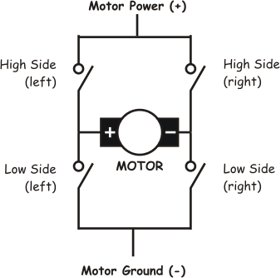
\includegraphics[width=\textwidth]{Motors/basic-bridge}

Controlar amb interruptors l'estat de HIGH i LOW podent fer veure que el motor està connectat en els dos sentits per tal de poder controlar la seva direcció. Aquest esquema també es pot realitzar mitjançant relés si no es volgués controlar la velocitat i la intensitat.

per controlar la velocitat a la qual fem girar el motor nesesitem fer el pont en transitors i controlar el dispar mitgagent honas PWM per tal de controlar el voltage que veu el motor: \smallskip

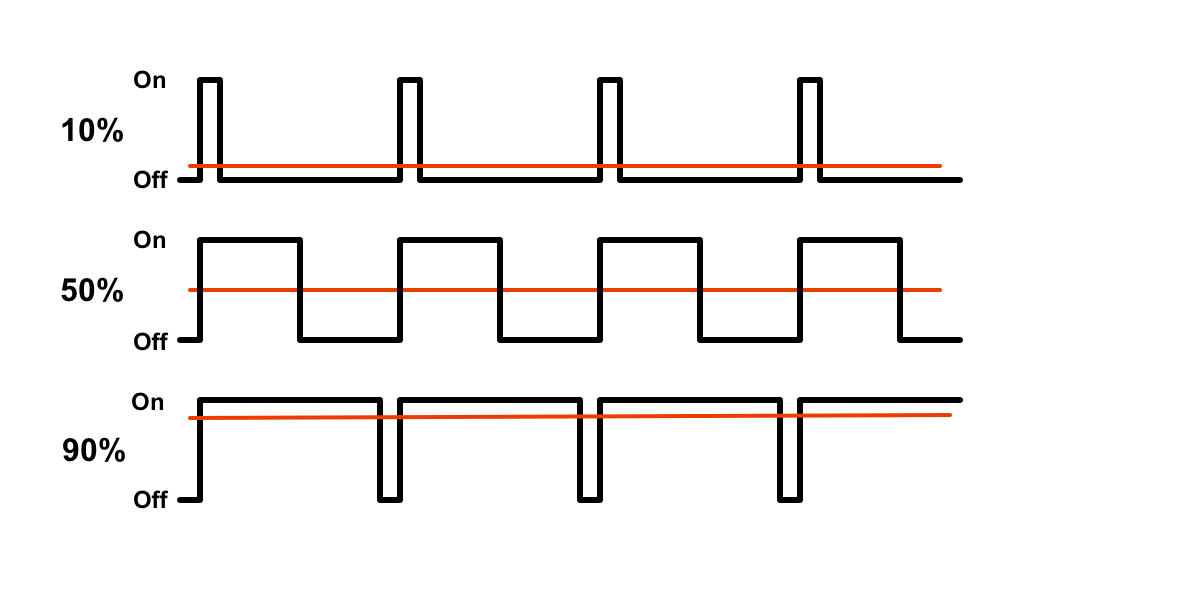
\includegraphics[width=\textwidth]{Motors/PWM}

Mitjançant una ona quadrada a una freqüència determinada, es podrà controlar el percentatge de l'ona que és el temps que l'ona es troba en estat HIGH i en LOW dins d'un mateix cicle. Es podrà donar doncs polsos amb el cicle complert a HIGH o complert a LOW lo suficientment ràpid com per que el motor treballi a voltatge constant, per variacions en la càrrega es pot variar la velocitat del motor, per tant es munten controls PID per tal d'anar adaptant la sortida del pont mantenint la velocitat controlada.

Amb el control de voltatge tindrem el control de la velocitat i el sentit. Pràcticament tindrem tot el control total del motor, encara que segueix havent el perill de cremar-lo. Per això es munta un segon sistema de control que controla la intensitat subministrada al motor per tal de tenir la força que crea la intensitat controlada. És munta doncs un PID per tal de poder saber la intensitat real que està arribant al motor per tal de modificar el cicle de l'ona per reduir-la o augmentar-la per tal de controlar la força realitzada pel motor.

Existeixen problemes amb el pont de potència, el pont en H. En el cas que volguéssim controlar el pont en forma de transistors i amb ones PWM, no ens podríem basar només en controlar els interruptors en creuat, ja que un motor està format per bobines i al tallar de cop la circulació de corrent el voltatge es podria disparar, arribant a cremar els transistors. Per tant cal controlar el pont mitjançant 4 sortides i no 2 com es donaria a entendre, a part s'hauran de connectar díodes de contrapolaritat entre el positiu i el negatiu del motor per a que deixi de fluir corrent invers. Les etapes d'aquest procés serien les següents:

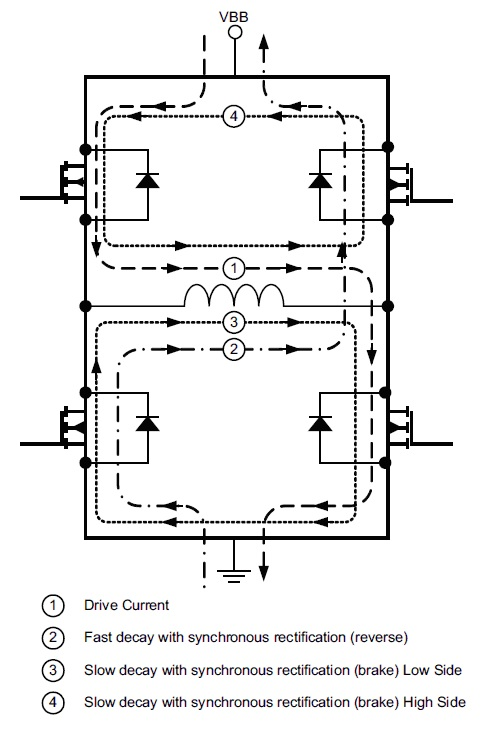
\includegraphics[width=\textwidth]{Motors/Hsteps}
\bigskip

\begin{enumerate}
    \item Control de corrent per polsos per tal de subministrar corrent al circuit. Recordar deixar el pont en H obert per facilitar el pas de corrent i que no \newline apareguin tensions molt altes que pugin cremar el pont. 
    \item Es deixarà que el corrent del motor passi pels díodes per tal de disminuir el corrent del motor i que el voltatge no es dispari i pugi cremar els transistors. Això succeirà si es manté una frenada progressiva del motor i una desacceleració. Es pot accelerar connectant els mosfets contraris per tal d'accelerar la frenada però pot produir una acceleració a l'invers. 
    \item La circulació de corrent per al estat LOW o HIGH es basa en deixar un dels dos mosfets inferiors o superiors activats per tal de provocar el bucle de corrent i desaccelerar ràpidament el corrent de motor.  
\end{enumerate}

\subsection{Motors de corrent altern}

En el control de motors de corrent altern la seva velocitat no ve definida pel voltatge que li apliquem directament sinó que ve definida per la freqüència de commutació de la xarxa. Per això existeixen dos maneres de controlar-ho; entrant a la xarxa per contactor que dóna directament el voltatge o bé en un circuit amb contactors que ens permet canviar el sentit de gir invertint una de la seves fases. En els cassos del trifàsics amb arrancada estrella-triangle que són les dues potències que pot tenir un motor, s'arrencarà per la part menys potent i anirà cap a la més potent amb el motor en marxa.


\subsubsection{Control mitjançant un variador de velocitat}
En el control per variació de velocitat necessitarem una font de corrent continu en el voltatge de pic del motor altern. Una vegada tinguem aquesta, muntarem un inversor trifàsic o monofàsic per tal d'emprar l'ona PWM i generar un pseudo-senyal sinusoïdal en el qual podrem controlar la seva freqüència, el seu voltatge i la intensitat de forma que puguem determinar la potència del motor per no cremar-ho i la freqüència per determinar el sentit i velocitat de gir.

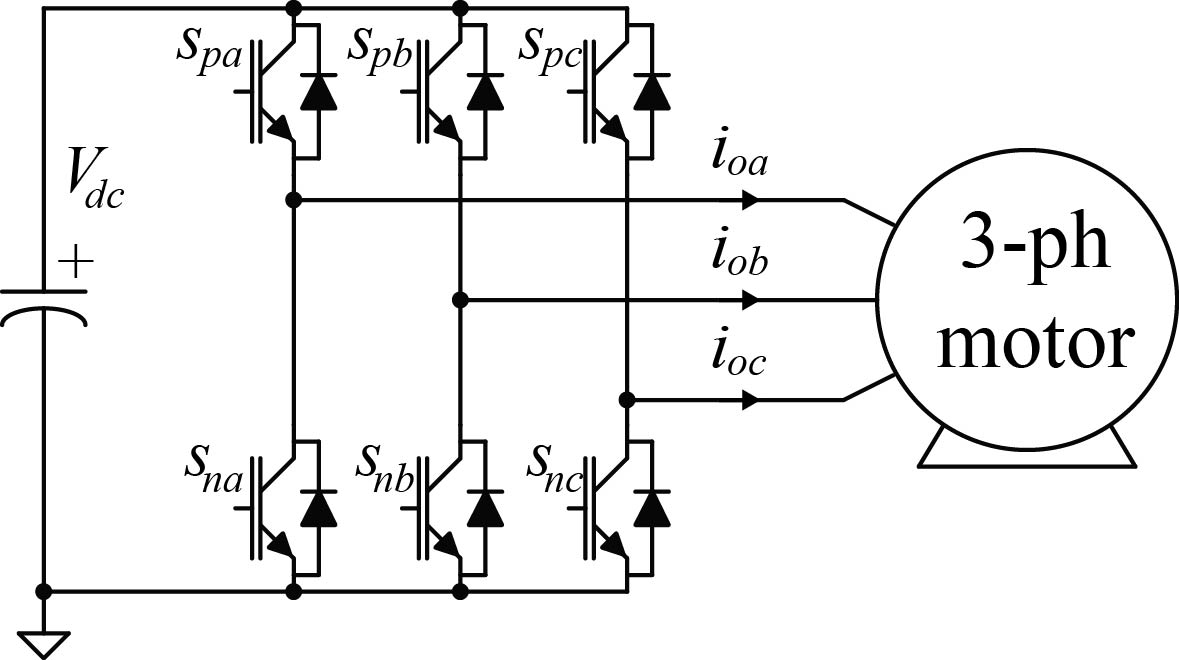
\includegraphics[width=\textwidth]{Motors/inverter}

A part de controla les variables en qüestió existeixen alguns paràmetres més que poden ser interessants com per exemple el fre per injecció de CC que consisteix en fer circular corrent continu en el motor per tal de generar un camp magnètic fix i produir una frenada molt forta del motor.

\subsection{control de motors pas a pas }

En el control de motors pas a pas disposem de bobines repartides pel motor amb connexió exterior, per norma general està composat per 2 bobinats alterns. El control normal és de llaç obert però també disposen de llaç tancat. El que fem per controlar aquest tipus de motor és activar les bobines des d'un microcontrolador fixant la posició del Stepper en una bobina o combinació d'aquestes conegut com a microstepping.

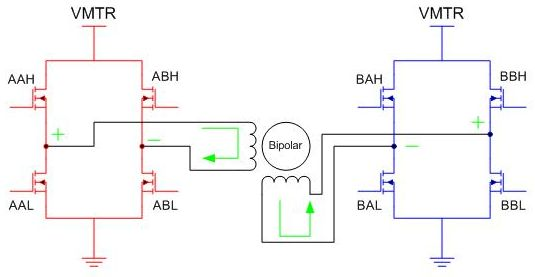
\includegraphics[width=\textwidth]{Motors/stepers.jpg}

Aquí només hem de controlar la intensitat que va a cada bobina per tal de no cremar-les. Una vegada controla la intensitat el que cal fer és invertir el voltatge de les bobines i les bobines activades, per tal d'anar canviant la posició del Stepper a la posició desitjada. Un problema comú és quan el motor està proper al parell que pot generar i es perden passos, és a dir, el motor es salta una bobina per culpa del parell resistiu que té en l'eix. La forma de solucionar-ho és aplicant un motor més potent o fent que el control sigui de llaç tancat. Un exemple d'un d'aquests motors en llaç obert és la impressora 3D.

El control dels ponts en H és molt similar al control que tenim en els motors de CC intentant mantenir una intensitat constant. Normalment s'utilitzen integrats per facilitar les feines com els DRV8825 \footnote{https://www.pololu.com/product/2133} o altres similars, aquests drivers el que fan és simplificar-nos el control en, enable per activar els bobinats de pas i direcció pel control. També podem configurar el microstepping fins a 1/32 o múltiples inferiors

\subsection{Controls de motors brushless}
Un motor brushless es controla d'una forma molt similar a un motor de CC però amb algunes complicacions. En comptes d'1 bobinat que va canviant per l'efecte de les escombretes, ara en tenim 3 i en comptes de escombretes per generar l'imant interior tenim un imant permanent. Això provoca que la velocitat vagi lligada als voltatges de les fases, però no pot ser constant ja que no s'inverteixen automàticament. S'ha d'invertir mitjançant l'electrònica i adaptar la freqüència a aquesta velocitat. Això provoca que els motors brushless hagin de tindre un sistema de control molt més complicat.

Hi ha una gran complicació a l'hora de saber la posició de l'eix per tal de poder calcular les commutacions a les bobines per seguir el moviment del motor. Això és un problema que moltes vegades es soluciona amb sensors a l'interior del motor, que és el sistema més eficaç. Es fan servir diversos mètodes per saber la posició aproximada de l'eix i així controlar la commutació de les fases.

\subsubsection{Etapa de potència}

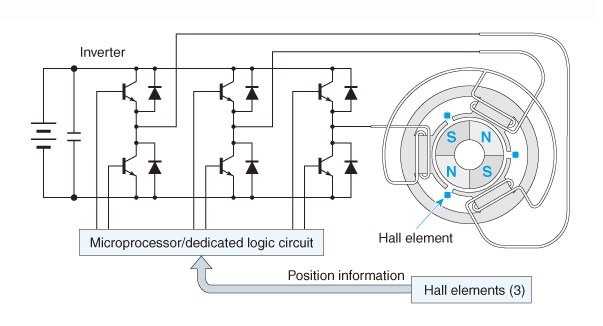
\includegraphics[width=\textwidth]{Motors/BLDC1}

A l'etapa de potència trobem un esquema molt similar als onduladors trifàsics. El nostre objectiu no és crear un senyal sinusoïdal sinó controlar impulsos de corrent continu que enviem al motor. Tenim el triple pont i podem connecta la fase que vulguem a a + i negatiu. Mitjançant el controlador disposem de 3 sensors opcionals d'efecte hall i el controlador hauria de ser capaç de mesurar la tensió de cada fase i la seva intensitat. Aquests controladors poden operar a diferents tensions i normalment treballen per tal de tirar el corrent generat al frenar el motor o a un activador per activar el corrent cap al sistema de control.
%en la eptapa de potenci trobem un esquema molt sismilar als onduladors trifacs dels motors de corrent altern, pero en aquet cas el nostre obgetiu no es crear una seudosinisuidal sino controlar els inpulsos de coorent continu que enviem al motor. tenim el triple pont i poden conectar la fase que volgem a a + i negetiu mitgenen el controlador disposem 3 sesors opcionas del efecta hall, i el controlador auria de ser capas de mesurar la tencio de cada fase i la seva intencitat. aquets controladors poden operar a difarentes tencions i normalemnt treballan amb grans intencitats, alguns del controladors apart disposens de una resistencia de descarga per tal de tirar el corrent de generat al frenar el motor o a un activador per activar el coorent cap el sistema de control,

\subsubsection{Oscil·lació de las fases}

En el cas de disposar de motors amb sensors d'efecte hall tindrem un punts de referència per saber en quin punt podem commutar les fases per obtenir la màxima eficiència i potència del motor. En canvi si el sistema de control el fem pel voltatge de la fase flotant estem pendents de la fase flotant per tal de saber en quin punt cal commutar les fases per que segueixi girant el motor.
%en el cas de diposer motors amb sensconrs de efecta hall tindrem un puts de per sapiger en quin punt podem comutar les fases por obtenir la maima eficencia i potencia del motor, en cavi si el sistema de control el fem per el voltage de la fase flotant estem pandets de la fase flotant per tal de sapiger en quin punt en de comuntar les fases per fer segi giratn el motor 

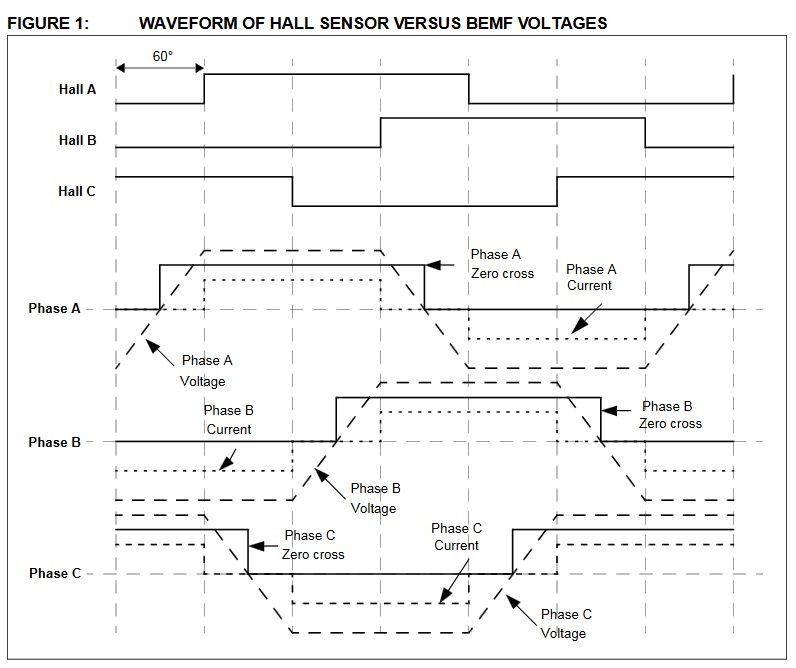
\includegraphics[width=\textwidth]{Motors/BLDC_DC_Motor_Sensorless_Trapezoidal_waveform}

En la part superior tenim els pins on el sensors d'efecte hall oscil·len determinant-se la forma del camp magnètic que tenim amb el rotor, per tal de conèixer la seva posició i saber quan commutar les bobines.

En canvi en els motors Sensorless hem de controlar el voltatge de la fase que penja, és a dir, quan estem alimentant les fases AB, la fase C queda lliure per poder capturar el voltatge i saber quan passa per 0 per activar la commutació. En el pas per 0 del voltatge de la fase voladissa per tal de detectar el canvi i coordinar la commutació.

Com es pot veure, els dos controlen la freqüència de commutació per fer accelerar el motor, ja que la velocitat d'aquests motors no es controla per la freqüència de gir, sinó pel voltatge de les fases. El control de la velocitat és el mateix que un motor de corrent continu amb escombretes depenent del voltatge de les seves fases, per això els transistors de l'etapa de potència els controlem amb un senyal PWM que defineix la velocitat del motor. En algunes aplicacions podria ser interessant calcular les revolucions a les quals gira el motor per fer-lo de llaç tancat. Per aquest tipus de motor no tendeix a trigar per aplicar càrrega sinó que demana un comú més alt d'amperes per tal de mantenir la velocitat amb molt poc o quasi nul amorrament, sempre que puguem gestionar la potència.
%com es pot veura com dels dos controla la frecuenci ade comutacio per fer acelarar el motor ja que la velositat de aquets motors no es controla per la frequencia de gir si no per el voltage de las pfases que saplien es a dir el control de la velositat es el matex que un motor deo corrent continu amb escoveta depedndre del voltage de las sevas fases, per aixo els trasistors de la etapa de potencia els controlaem amb PWm per definir la velositat del motr, en algunes paplicacion podria ser interantant calcular les rom del gira el motor per ferlo de llas tancat per aquet tipus de motor no tendex a amorarse al plicar carga sino que demana un comun mes alt de ambpers per tal de mentarni la velociat amb molt poc o casi null ammorrament sempre que pugem gestionar la potencia. 

\subsubsection{CPU de control}

Existeixen múltiples maneres de controlar un motor brushless. Cada marca té la seva pròpia manera de controlar-ho i tenen petites variacions, encara que totes tendeixen a una idea principal de control. En el cas en el que ens basem es mostra un diagrama de blocs d'una versió comercial de Texas Instruments.

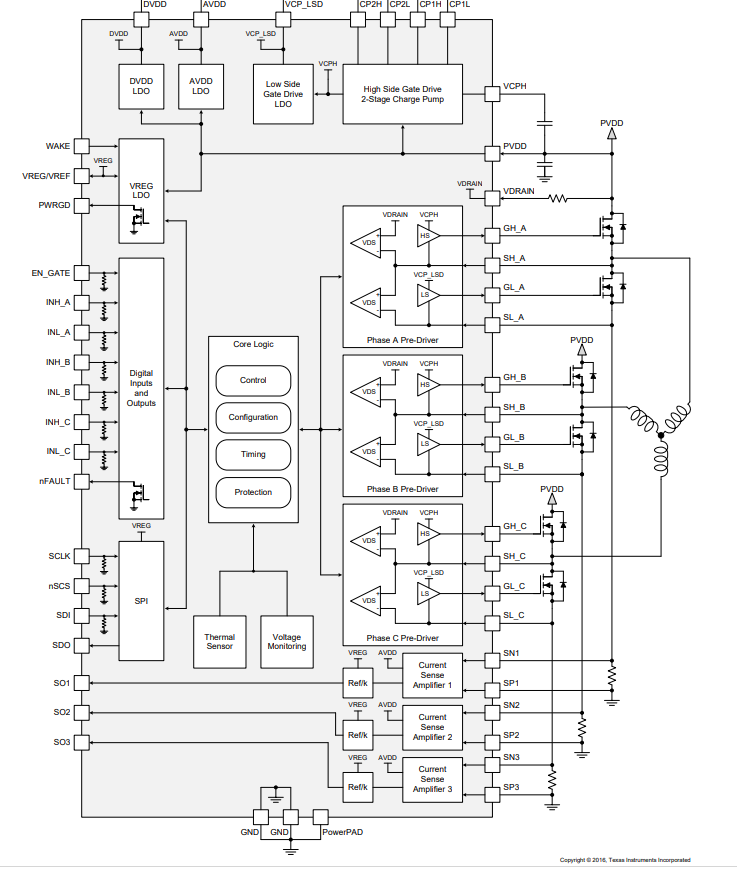
\includegraphics[width=\textwidth]{Motors/controlsquematic}

\textbf{Control dels transistors mosfet}\newline \smallskip

Si ens mirem els GH-A a sh-a, gl-a i sl-a controla una branca de l'inversor trifàsic que es composa de dos mosfets. Del motor tenim l'entrada sh-a i sl-a que estan connectades poder elevar la tensió de forma que el mosfet pugui obrir l'entrada de control, de forma que la tensió entre el gh-a i el sh-a es mantingui per sobre, suficient per mantenir el mosfet obert i controlar que tinguem curctcircuit. Per això mesurem la tensió entrel VDRAIN i el sh-a i comprovem la caiguda de tensió, de ser molt elevada tallem. També incorpora una mesura de corrent per fase, en la part inferior tenim el sn1, sp1 amb un shun per determinar la caiguda de tensió i saber la intensitat que circula per cada base.
%si ens mirem els GH-A sh-a gl-a sl-a controla una braca del inversor trifasic que es composa de dos mosfets de el motor tenim la intrada sh-a i sl-a que estan conectades per poder elevar la tencio de forma que el mosfet pugi obrir la entrada de cotnrol de forma que la tencia entre el gh-a i el sh-a es mentigi per sobre lo sufent per mentenir el mosfet obert i contolar que no tignem un corcirquit, per aixo mesurem la tencio entre el VDRAIN i el sh-a i comprovem la caiguda de tencio si es mol elevada tallem. tambe incormpera una mesura de corrent per fase, en la part inferor tenim el sn1 sp1 amb un shun per determinar la caguda de tencio i saver la intencitat que cirlula per cada fase. 

\textbf{Voltatges i fonts aïllades} \newline \smallskip

Per poder obrir el mosfet necessitem donar una tensió entre la gate i el source determinada per la conducció del mosfet. Hem de disposar d'una font de més voltatge que la font de la bateria principal, això ens provoca que s'hagin de fer fonts flotants per poder contrlar els mosfets. Això ja ho fa internament el controlador, però algunes tècnices serien carregar un condensador connectat entre el gate i el source i descarregar-ho per obrir el mosfet sempre que el temps d'obertura sigui petit i no descarreguem el condensador. A part hem de controlar la intensitat que necessiten els mosfets per forçar un tret ràpid, arribant a ser de 2A més o menys, i la mateixa en negatiu. En la part superior poden observar-se els condensadors que es fan servir per la porta d'alta i la font de conversió.

%per poder obrir el mosfet nesesitem donat una tesio entre la gete i el souce determinada per en conducio el mosfets de Higs em de disposatr de una font de mes voltage que la font de la bateria prisipal, aixo ens proboca que agem de fer fonts folotans per poder controlar els mosfets axo ga en ho fa internamen el contorlador pero algunes tecnices seria caregant un condensador que esta conecttat entre la surce i la gate i descagarlo per obrir el mosfet senpre que el tems de obertura segi petit i no descargem el condesador, apat emb de ocntolar la intacitat que domes els mofets per forcar un dispar rapid poden der de 2A mes o menso i la matexa en negatiu, en la part superior oden oberser els dos condesadors que es fan servir per la porta de alta, i la font de conversio\bigskip

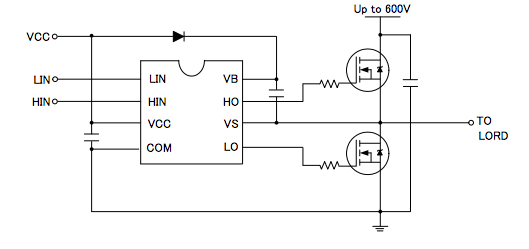
\includegraphics[width=\textwidth]{Motors/600-V-HighLow-Side-Gate-Driver-1427853331}

Aquí podem veure una mica aquest tipus de font. Ens centrarem en el VB, HO i VS que són la part interessant, ja que treballen per sobre del voltatge de HIGH voltatge. En estat de repós el H0 està connectat a massa i el corrent pot fluir des de Vcc fins a VS, de forma que el condenasdor queda carregat. Quan activem el tret del mosfet, el VB es connecta amb el HO de forma que tenim la tensió de la font en la porta del mosfet. Això provoca el tret del transistor i ens permet activar la porta i començar a conduir. Al conduir VS s'eleva per sobre VCC elevant el voltatge del condensador fins que el díode talli i ens quedi una font de VCC en el condensador per sobre la tensió del drenador del mosfet mantenint-lo obert. Al tancar-ho, el que fem és connectar-ho a massa i el díode i la font tornen a carregar el condensador per tornar-ho a tenir preparat. La resistència de la porta és perquè el condensador no es descarregui massa ràpid, arribant a cremar el mosfet limitant el corrent de la gate.
%aqui podem veura una mica quets tipus de font, ens centrerem el el VB HO VS qu son la pet interanet ga que trevalles per sobre del voltage de higvoltag, en estat de repos el H0 esta conectat a massa i el corrent pot fluit desde el vcc fins al vs de forma que el condesador queda carregat, cuan activem el dipsar el vb es connecta amb el HO de forma eu tenim la tencio de la font en la porta del mosfet aixo proboca el dipar del transistor i ens parment activar la porta i comensar a conduir, al cunduir vs saleva per sobre vcc elevant el voltage del condesador i fine que el diodi talli i ens queda una font de VCC en el condesador per sobre la tensio del drenador del mosfet manteninlo obert, al tancarlo el que fem es connectart Ho a masa i el diode i la font tornen a carregar el condesador per tornarlo a tenir preparar. la resitecia de la porta es per que elk condesador no es descare masa rapid poden cremar el mosfet limitat la corrent de la gate
 
 \textbf{Mètodes de control}\newline \smallskip
 
 Aquí si és on hi ha una àmplia diversitat entre marques i models, des de diferents interfícies de control, fins a disponibilitat d'entrades digitals, analògiques, PWM o comunicacions com CAN, SPI o Serial entre moltes més. Poden ser tant diversos que ens hem de mirar un producte en concret per saber com s'han de controlar. També disposen d'una unitat de processament per a les entrades corresponents o les comunicacions per tal de controlar tots aquests elements i  fer girar el motor com s'espera. 
 % aqui si que tenim un molt molt divers esntre marques i models comentails son la intefaces de control dels alemnts poden diposar de entredas digitals, analogicas pwm o mcomunicaicons com can, spi o serial entre moltes mes, poden ser tan diversos que ens em de mira run producte en conecnte per saver com san de controlar inclun estre marcas poden ser molt diverses,  tambe diposem de una unitat de prosesement CPU per amb les entrades correnspoents o les comunicacions controlar tots aquets elements i fer girar el motor com saspera. 
 
 \textbf{Característiques extres}
 
 Alguns controladors porten algunes característiques que poden ser interessant, com el control de l'alimentació de HV. Alguns ens permeten muntar un relé transistor per activar el HV. Podria ser interessant per no tenir tot el temps el circuit de potència connectat al motor. També alguns disposen d'una sortida per una resistència de crema, és a dir, en el cas que utilitzem el motor per frenar generarà una intensitat de sortida cap al HV. Si no la volem gestionar, és pot activar una resistència que actuï com a dissipador. També controlar la intensitat d'entrada al convertidor i controlar les resistències per tal de no injectar corrent al HV, entre altres funcions interessants. 

 \section{Elecció del motor brushless per al CVE}

Em decanto pels motors brushless pel prototip del controlador de vehicles elèctrics que tenim pensat implementar de forma teòrica. Els principals avantatges que ens donen aquest tipus de motor es llisten seguidament:

\begin{itemize}
    \item Major nombre de RPM, ja que no existeix pràcticament fregament. No disposen do commutació interna i només ens limitaria la commutació electrònica i el disseny mecànic del propi motor.
    \item No disposa de bobinat en l'interior del motor ni escombretes que provoquin fregament arribant a eficiències molt altes per sobre del 90\%. Això provoca que pràcticament no dissipen energia en forma de calor, donant una major autonomia de la bateria i menor desgast al no estar sotmès a altes temperatures.
    \item Major potència ja que no hem de crear els imants en el centre i amb uns imants permanent molt potents podem aconseguir entregues de potència molt altes, amb un pes molt baix com per exemple el Turnigy RotoMax 150cc Size Brushless que amb un pes de 2,3Kg aconsegueix una potència de 9,8Kw.
    %magor potencia ja que no em de crear els imans en el centre i amb uns impans permantats molt potens podem acosegir entregas de potencia molt altes amb un pes molt baix com peratgemple el Turnigy RotoMax 150cc Size Brushless  que amb un pes de 2,3kg aconsegim una potencia de 9,8 kw 
    \item Voltatges d'accionament reduïts. No en tots els casos, però per norma general aquests motors treballaran per sota els 60V. Això ens facilitarà el disseny d'una bateria es facilitarà el treball amb l'alt voltatge ja que estarem parlant de valors de 400V com en els d'alterna.
\end{itemize}

Tots aquests paràmetre ens porten a seleccionar aquest tipus de motor per al disseny del nostre controlador. Tot i que amb aquest tipus de motor la part més complex és el ESC que serà l'encarregat de controlar l'excitació dels camps de maneig per provocar el gir del motor. Tindrem avantatges extres ja que són un tipus de motor que molt fàcilment els podem convertir en generadors i tenint una eficiència alta podrem aprofitar per la frenada regenerativa per tal d'intentar millorar l'eficiència del VE. 




%%%%%%%%%%%%%%%%%%%%%%%%%%%%%%%%%%%%%%%%%%%%%%%%%%%%%%%%%%%%%%%%%%%%%%%%%%%%%%




% A PARTIR DE AQUI TODO MOVIDO AL VESC!!!!!!



%%%%%%%%%%%%%%%%%%%%%%%%%%%%%%%%%%%%%%%%%%%%%%%%%%%%%%%%%%%%%%%%%%%%%%%%%%%%%

